\chapter{Get started with \LaTeX\ }
\label{c:GetStarted}
Three common font styles in this text: 
\begin{itemize}
    \item \textbf{Item1}: \textit{Italic中文123}     
    \item \textbf{Item2}: \textbf{Bold中文123}
    \item \textbf{Item3}: \textsl{slant中文123}
\end{itemize}

About the advance latex grammer see the next section \ref{s:AdvancedFeatures}.


\section{\LaTeX\ Adavanced Features}
\label{s:AdvancedFeatures}
The following features would be introduced in the coming subsections:
\begin{itemize}
    \item SubSection \ref{ss:Figure}: \hyperref[ss:Figure]{\textbf{Figure}}
    \item SubSection \ref{ss:VerbUsage}: \hyperref[ss:VerbUsage]{\textbf{Verb}}
    \item SubSection \ref{ss:VerbUsage}: \hyperref[ss:VerbUsage]{\textbf{Verb}}
    \item SubSection \ref{ss:Enumeration}: \hyperref[ss:Enumeration]{\textbf{Enumeration}}
    \item SubSection \ref{ss:Table}: \hyperref[ss:Table]{\textbf{Table}}
    \item SubSection \ref{ss:CodeDisplay}: \hyperref[ss:CodeDisplay]{\textbf{Code Display}}
    \item SubSection \ref{ss:Math}: \hyperref[ss:Math]{\textbf{Math}}
    \item SubSection \ref{ss:Algorithms}: \hyperref[ss:Algorithms]{\textbf{Algorithms}}
\end{itemize}

%==========================================================================================
\subsection{Figure}
\label{ss:Figure}
\begin{figure}[htpb!]
  \centering
    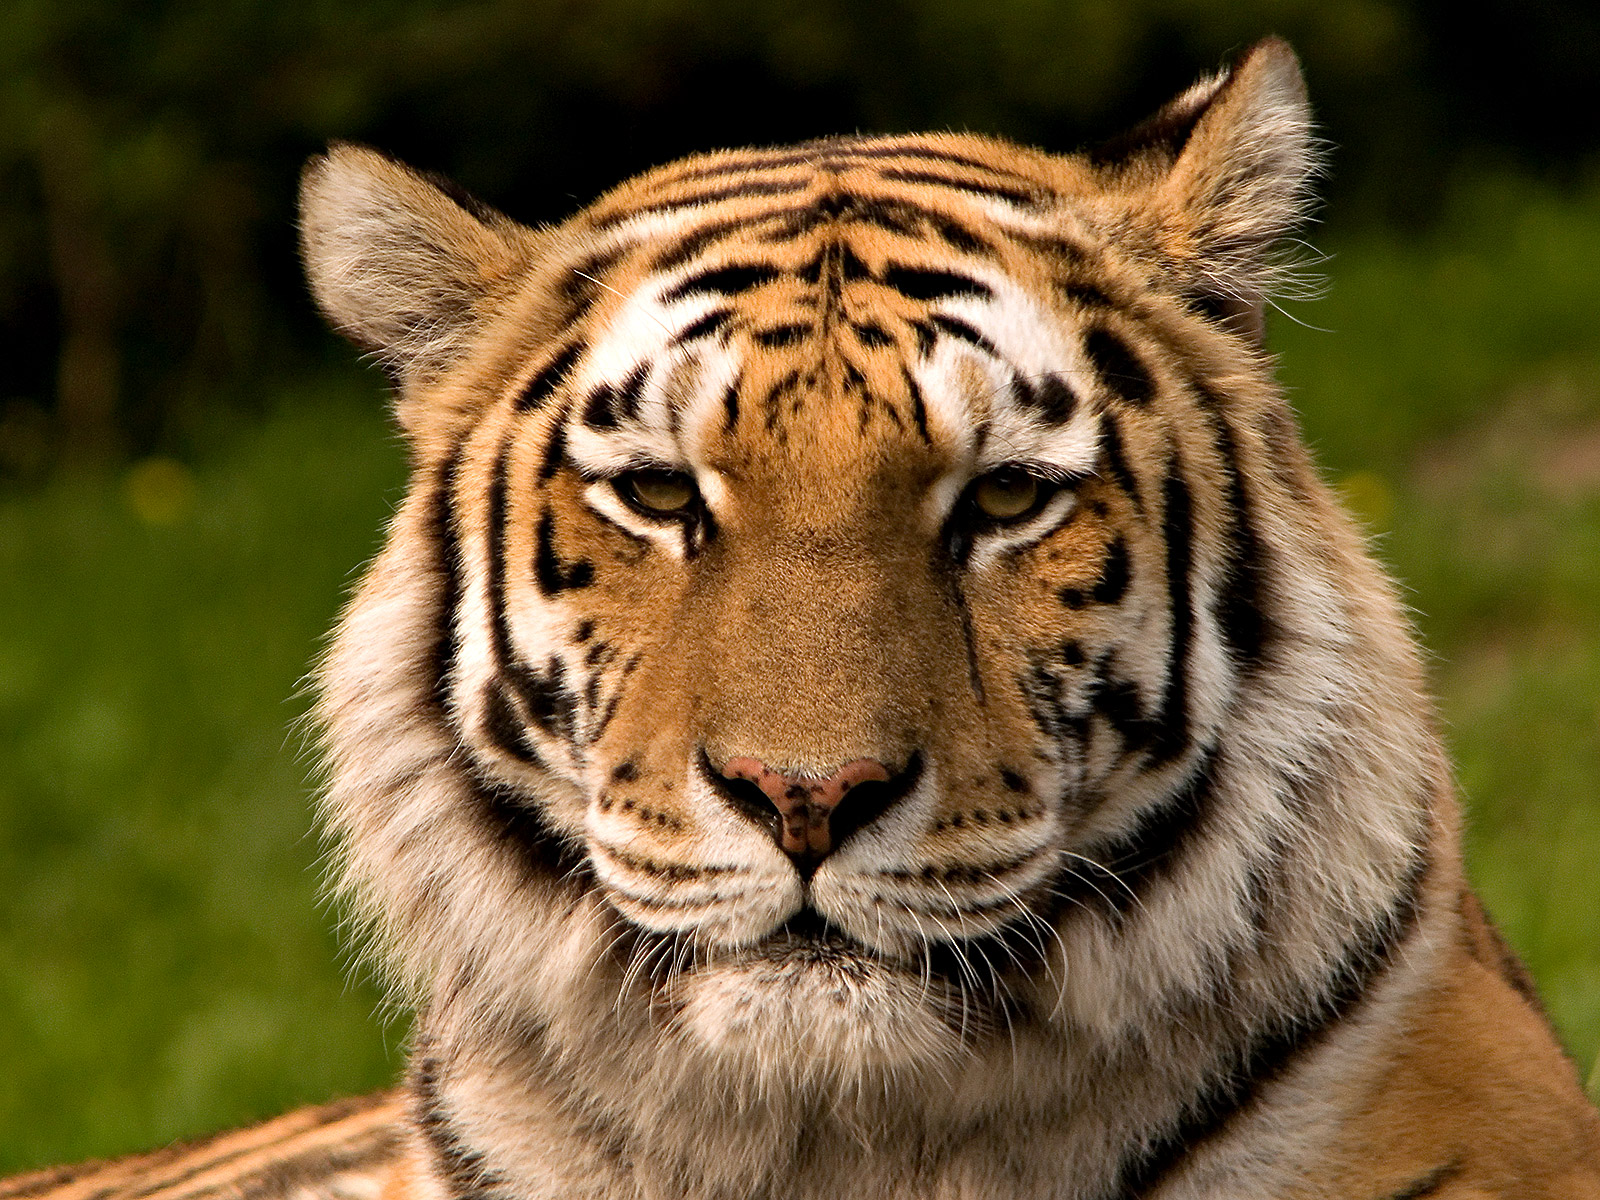
\includegraphics[width=0.5\textwidth]{fig/tiger.jpeg}
    \caption{\label{fig:tiger}A picture of a tiger.}
\end{figure}

Figure~\ref{fig:tiger} is a picture of a tiger.


%==========================================================================================
\subsection{Table}
\label{ss:Table}

\href{http://en.wikibooks.org/wiki/LaTeX/Tables}{Table examples on WIKIBOOKS}.

\begin{table}[htpb]\begin{center}
\caption{Table Example 1}
\begin{tabularx}{8cm}{llX}
\hline
Start & End  & Character Block Name \\
\hline
3400  & 4DB5 & CJK Unified Ideographs Extension A \\
4E00  & 9FFF & CJK Unified Ideographs \\
\hline
\end{tabularx}
 \end{center}\end{table}

\begin{table}[htpb]\begin{center}
\caption{Table Example 2}
\begin{tabular}{llr}
\hline
\multicolumn{2}{c}{Item} \\
\cline{1-2}
Animal & Description & Price (\$) \\
\hline
Gnat  & per gram & 13.65 \\
      & each     &  0.01 \\
Gnu   & stuffed  & 92.50 \\
Emu   & stuffed  & 33.33 \\
Armadillo & frozen & 8.99 \\
\hline
\end{tabular}
 \end{center}\end{table}
 
 \begin{table}[htpb]\begin{center}
	\label{t:prefix-table}
	\caption{Table Example 3}
	\renewcommand{\arraystretch}{1.0}
	\begin{tabularx}{300pt}{|c|X| }
		\hline
		\multirow{1}{*}{\textbf{Allocation}} &
		Allocation, Element, Type, Script 
		\\ \hline\hline
		%------------------------------
		\multirow{6}{*}{\textbf{Data Types}} &
        Byte2, Byte3, and Byte4\\ &
        Float2, Float3, Float4\\ &
        Int2, Int3, Int4\\ &
        Long2, Long3, Long4\\ &
        Matrix2f, Matrix3f, Matrix4f\\ &
        Short2, Short3, Short4
        \\ \hline\hline
		%------------------------------
		\multirow{4}{*}{\textbf{Graphics}} &
		Mesh\\&
		ProgramFragment, ProgramRaster\\&
		ProgramStore, ProgramVertex\\&
		RSSurfaceView
		\\ \hline
		%------------------------------
	\end{tabularx}
\end{center}\end{table}

\begin{table}[htpb]\begin{center}
\caption{Table Example 4}
\begin{tabular}{|l|l|l|}
\hline
\multicolumn{3}{|c|}{Team sheet} \\
\hline
Goalkeeper & GK & Paul Robinson \\ \hline
\multirow{4}{*}{Defenders} & LB & Lucus Radebe \\
 & DC & Michael Duberry \\
 & DC & Dominic Matteo \\
 & RB & Didier Domi \\ \hline
\multirow{3}{*}{Midfielders} & MC & David Batty \\
 & MC & Eirik Bakke \\
 & MC & Jody Morris \\ \hline
Forward & FW & Jamie McMaster \\ \hline
\multirow{2}{*}{Strikers} & ST & Alan Smith \\
 & ST & Mark Viduka \\
\hline
\end{tabular}
 \end{center}\end{table}
 
 \begin{table}[htpb]\begin{center}
\caption{Table Example 5}
 \begin{tabular}{l*{6}{c}r}
Team              & P & W & D & L & F  & A & Pts \\
\hline
Manchester United & 6 & 4 & 0 & 2 & 10 & 5 & 12  \\
Celtic            & 6 & 3 & 0 & 3 &  8 & 9 &  9  \\
Benfica           & 6 & 2 & 1 & 3 &  7 & 8 &  7  \\
FC Copenhagen     & 6 & 2 & 1 & 2 &  5 & 8 &  7  \\
\end{tabular}
 \end{center}\end{table}

%==========================================================================================
\subsection{Verb}
\label{ss:VerbUsage}
Let's take a overview on how to type special characters:\\
\verb|<FRAMEWORKS_BASE>/graphics/java/android/renderscript|\\\footnote{Path of <APP\_intermediates>: <ANDROID\_ROOT>/out/target/common/obj/APPS/APPNAME\_intermediates/}
You could also go back to the beginning of the chapter by the \hyperref[c:GetStarted]{\textbf{hyperref}}.

%==========================================================================================
\subsection{Enumeration}
\label{ss:Enumeration}
\begin{enumerate}
\item Enumerated Item1
\item Enumerated Item2
\item Enumerated Item3
\end{enumerate}

%==========================================================================================
\subsection{Code Display}
\label{ss:CodeDisplay}

\lstset{
	language=C++,
	stringstyle=\rmfamily,
	commentstyle=\itshape\color[rgb]{0.133,0.545,0.133},
	showstringspaces=false,
	basicstyle=\ttfamily\scriptsize,
	numberstyle=\tiny,
	numbers=left,
	stepnumber=1,
	numbersep=10pt,
	tabsize=2,
	breaklines=true,
	prebreak = \raisebox{0ex}[0ex][0ex]{\ensuremath{\hookleftarrow}},
	breakatwhitespace=false,
  	columns=fixed,
  	upquote=true,
  	extendedchars=true,
	xleftmargin=2em,
	xrightmargin=.5em,
	escapeinside={(*@}{@*)},
    mathescape=false,
}
Here is a "Hello, DanDing." example:
\begin{lstlisting}[style=nonumbers] 
void main(int argc, char **argv)
{
    printf("   ˊ_> ˋ  ");
}
\end{lstlisting}


Another example with line numbers:
\begin{lstlisting}
void main(int argc, char **argv)
{
    printf("   ˊ_> ˋ  ");
}
\end{lstlisting}

Matlab example:

\definecolor{dkgreen}{rgb}{0,0.6,0}
\definecolor{gray}{rgb}{0.5,0.5,0.5}
\lstset{language=Matlab,
   keywords={break,case,catch,continue,else,elseif,end,for,function,
      global,if,otherwise,persistent,return,switch,try,while},
   basicstyle=\ttfamily,
   keywordstyle=\color{blue},
   commentstyle=\color{red},
   stringstyle=\color{dkgreen},
   numbers=left,
   numberstyle=\tiny\color{gray},
   stepnumber=1,
   numbersep=10pt,
   backgroundcolor=\color{white},
   tabsize=4,
   showspaces=false,
   showstringspaces=false}

\begin{lstlisting}
function y = demo(x) % This is a comment.
   str = 'hello there';
   y = x + 1;
end
\end{lstlisting}

%==========================================================================================
\subsection{Math}
\label{ss:Math}
\begin{itemize}
    \item Inline mode:\\
The solution to $\sqrt{x} = 5$ is $x=25$.
    \item Display mode:\\
The solution to \[\sqrt{x} = 5\] is \[x=25.\]
    \item Numbered mode:
\begin{equation}
2+2=4
\end{equation}
    \item Non-numbered:
\begin{equation*}
2+2=4
\end{equation*}
    \item Aligning:
\begin{align*}
2x^2 + 3(x-1)(x-2) & = 2x^2 + 3(x^2-3x+2)\\
&= 2x^2 + 3x^2 - 9x + 6\\
&= 5x^2 - 9x + 6
\end{align*}
     \item Fractions:
\[
 \frac{n!}{k!(n-k)!} = \binom{n}{k}
\]
    \item Matrix:
\[
 A_{m,n} =
 \begin{pmatrix}
  a_{1,1} & a_{1,2} & \cdots & a_{1,n} \\
  a_{2,1} & a_{2,2} & \cdots & a_{2,n} \\
  \vdots  & \vdots  & \ddots & \vdots  \\
  a_{m,1} & a_{m,2} & \cdots & a_{m,n}
 \end{pmatrix}
\]
\end{itemize}
\href{http://en.wikibooks.org/wiki/LaTeX/Mathematics}{More examples on WIKIBOOKS}.


%==========================================================================================
\subsection{Algorithms}
\label{ss:Algorithms}
\begin{algorithm}[h]                      % enter the algorithm environment
\caption{Calculate $y = x^n$}          % give the algorithm a caption
\label{alg1}                           % and a label for \ref{} commands later in the document
\begin{algorithmic}                    % enter the algorithmic environment
    \Require $n \geq 0 \vee x \neq 0$
    \Ensure $y = x^n$
    \State $y \Leftarrow 1$
    \If{$n < 0$}
        \State $X \Leftarrow 1 / x$
        \State $N \Leftarrow -n$
    \Else
        \State $X \Leftarrow x$
        \State $N \Leftarrow n$
    \EndIf
    \While{$N \neq 0$}
        \If{$N$ is even}
            \State $X \Leftarrow X \times X$
            \State $N \Leftarrow N / 2$
        \Else[$N$ is odd]
            \State $y \Leftarrow y \times X$
            \State $N \Leftarrow N - 1$
        \EndIf
    \EndWhile
\end{algorithmic}
\end{algorithm}
\href{http://en.wikibooks.org/wiki/LaTeX/Algorithms_and_Pseudocode}{More examples on WIKIBOOKS}.

